\documentclass[12pt]{article}
\usepackage{amsthm}
\usepackage{bbm}
\usepackage{amssymb}
\usepackage{mathtools}
\mathtoolsset{showonlyrefs,showmanualtags}
\usepackage{etoolbox}
% \usepackage{booktabs}
% \usepackage{url}
\usepackage{setspace}
\usepackage[margin=1in]{geometry}
\usepackage{authblk}
\usepackage{natbib}
% \usepackage[page]{appendix}
\usepackage[nomarkers,nolists]{endfloat}
\usepackage{graphicx}
% \usepackage{caption}
% \usepackage{subcaption}
\usepackage{tikz}
\usetikzlibrary{calc}
\usepackage{subfig}
\usepackage{enumitem}
\usepackage{array} % tables with fixed width and alignment
\usepackage{chngpage} % for the too long table at the end
\usepackage{xr} % reference proofs in suppl material
\DeclareMathOperator{\AUC}{AUC}
\DeclareMathOperator{\V}{Var}
\DeclareMathOperator{\cov}{Cov}
\DeclareMathOperator{\corr}{Corr}
\DeclareMathOperator{\sd}{sd}
% \renewcommand{\t}[1]{\tilde{#1}}
\newcommand{\h}[1]{\hat{#1}}
\newcommand{\I}{I}
% \newcommand{\partiall}[1]{\frac{\partial}{\partial #1}}
% \newcommand{\gm}{\theta}
\newcommand{\E}{E}
\renewcommand{\P}{P}
% \newcommand{\mean}[1]{\overline{#1}}
% \newcommand{\sel}[1]{#1^*}
% \newcommand{\biasratio}{b}% {$(E|S_1-S_2|)^2/\E(S^2)$}
\newcommand{\cind}{\perp \!\!\! \perp}
\newcommand{\aucindiv}{\theta_{11}}%{\AUC}
\newcommand{\aucpop}{\theta_{12}}%{\AUC_{\cind}}
\newcommand{\aucindivhat}{\hat{\theta}_{11}}%{\AUC}
\newcommand{\aucpophat}{\hat{\theta}_{12}}%{\AUC_{\cind}}
\newcommand{\kernel}{\psi}
\newcommand{\Kernel}{\psi}
\newcommand{\B}{B}
% \newcommand{\W}[1]{X_{#1},Y_{#1}}
\newcommand{\W}[1]{W_{#1}}
\newcommand{\bnd}{a}
% \renewcommand{\V}{c_{00}}
\newcommand{\seqspace}{V}%{c_{00}}
\renewcommand{\d}{\phi}
\newcommand{\Pind}{P_{\cind}}
\newcommand{\A}[1]{P(A^{(n)}_{#1})}
\newtheorem{theorem}{Theorem}
\newtheorem{proposition}[theorem]{Proposition}
\newtheorem{lemma}[theorem]{Lemma}
\newtheorem{corollary}[theorem]{Corollary}
\makeatletter
\def\input@path{{../input/}{../figs/}}
\graphicspath{{../figs/}}
\makeatother
\newcommand{\PreserveBackslash}[1]{\let\temp=\\#1\let\\=\temp}
\newcolumntype{C}[1]{>{\PreserveBackslash\centering}p{#1}}
\newtoggle{commenttoggle}
\togglefalse{commenttoggle}
\newcommand{\comment}[1]{
  \iftoggle{commenttoggle}{
    {\normalsize{\color{red}{ #1}}\normalsize}
  }
  {}
}
\externaldocument{manuscript}
\doublespacing
\title{Supplementary Material for ``The Population and Personalized AUCs''}
\author[1]{Haben Michael}
\author[2]{Lu Tian}
\affil[1]{University of Massachusetts}
\affil[2]{Stanford University}
\date{}

\begin{document}

% % \maketitle
% % \noindent\textsc{Abstract:} We consider two generalizations of the AUC to accommodate
% % clustered data. We describe situations in which the two cluster AUCs
% % diverge and other situations in which they coincide. We apply the
% % results to data collected on urban policing behavior.\\
% % \textsc{Keywords:} AUC, Confounding, Clustered data, Simpson's paradox



%   \begin{proof}[Proof of Proposition \ref{proposition:aucpop}]
%     \begin{enumerate}
%     \item By the LLN $\I^2/MN \to 1/(\E (M)\E (N))$ almost surely and by Lemma \ref{corollary:convergence} $\sum_{i,j}\Kernel_{ij}/\I^2 \to \E \Kernel_{12}$ almost surely. Conditioning on the sample,
%       \begin{align}
%         \E \kernel(\xi_\I,\eta_\I) &= \E( \E (\kernel(\xi_\I,\eta_\I) \mid (X_1,Y_1,M_1,N_1),\ldots,(X_\I,Y_\I,M_\I,N_\I))\\
%                                    &= \E\left(\frac
%                                      {\sum_{1\le i,j\le\I}\sum_{1\le k\le M_i,1\le l\le N_j}\kernel(X_{ik},Y_{jl})}
%                                      {\sum_{i=1}^\I M_i \sum_{i=1}^\I N_i} \right)\\
%                                    &= \E\left(\frac{\sum_{1\le i,j\le\I}\Kernel_{ij}}{\sum_{i=1}^\I M_i \sum_{i=1}^\I N_i} \right) \to \frac{\E\Kernel_{12}}{\E (M) \E (N)}=\aucpop.
%       \end{align}
%       The limit is justified since $\sum_{i,j}\psi_{i,j}/(\sum_i M_i\sum_i N_i)\le 1$. %dominated convergence, given the boundedness of $\I^2/MN$ and moment condition on $\Kernel$.

%     \item The second part follows on showing that $(\xi_\I,\eta_\I)\to (\xi_\infty,\eta_\infty)$ setwise. % \comment{if arguing $\theta_{12}(P_\I)\to\theta_{12}(P_\infty)$ need to show $P_\I$ concentrates on a continuity set of $P_\infty$.}
%       For $a,b\in\mathbb{R}$, by a similar argument as above,
%       \begin{align}
%         \P(\xi_\I<a,\eta_\I<b) &=\E\left(\frac
%                                      {\sum_{1\le i,j\le\I}\sum_{1\le k\le M_i,1\le l\le N_j}\{X_{ik}<a,Y_{jl}<b\}}
%                                  {\sum_{i=1}^\I M_i \sum_{i=1}^\I N_i} \right)\\
%                                &\to \frac{\E\left(\sum_{k=1}^{M_1}\{X_{1k}<a\}\right)}{\E (M)}
%                                  \frac{\E\left(\sum_{l=1}^{N_1}\{Y_{1l}<b\}\right)}{\E (N)}.
%       \end{align}
%       The probability of sampling an element from a cluster of size
%       $M=m$ given an initial segment of $\I$ samples
%       $(X_1,Y_1,M_1,N_1),\ldots,(X_\I,Y_\I,M_\I,N_\I),$ is
%       $\frac{m\sum_{i=1}^\I\{M_i=m\}}{\sum_{i=1}^\I M_i}$. Along almost
%       any sequence of samples as $\I\to\infty$ this relative frequency
%       tends to $\frac{m\P(M=m)}{\E (M)}$. Therefore
%       \begin{align}
%         \P(\xi_\infty < a) &= \sum_{m=1}^\infty\P(\xi_\infty < a \mid \xi_\infty\text{ is sampled from a cluster of size }m)\cdot\\
%         &\hspace{.5in}\P(\xi_\infty\text{ is sampled from a cluster of size }m)\\
%                            &= \sum_{m=1}^\infty\frac{1}{m}\sum_{k=1}^m\P(X_{1k}<a\mid M=m)\frac{m\P(M=m)}{\E (M)}\\
%                            &=\frac{1}{\E M}\sum_{m=1}^\infty\sum_{k=1}^m\P(X_{1k}<a\mid M=m)\P(M=m)\\
%         &=\frac{1}{\E (M)}\E\left(\sum_{k=1}^M\{X_{1k}<a\}\right).
%       \end{align}
%       Analogously,
%       $$
%       \P(\eta_\infty < a)=\frac{1}{\E (N)}\E\left(\sum_{l=1}^N\{X_{1l}<a\}\right).
%       $$
%       The product is the limit of
%       $\P(\xi_\I<a,\eta_\I<b)$ given above.
%     \end{enumerate}
%   \end{proof}
%     The following lemma gives a convergence result for a two-sample $U$-statistic with kernel of degree $(1,1)$ where the data is paired. The corresponding definitions and result for independent samples is given in, e.g., \citet{lee2019}. Let $\seqspace$ denote the space of finite sequences.%\comment{Need to define $V$, the space where $X,Y$ lie. These are vectors of variable length so $V$ should be at least as big as $c_{00}$}

%   %   \begin{lemma}\label{lemma:hajek} Given a sample $(X_0,Y_0),(X_1,Y_1),\ldots,(X_\I,Y_\I)$ on
%   %   $\seqspace\times\seqspace$ IID according to $\P$ and a
%   %   function $\Kernel: \seqspace\times\seqspace \to \mathbb{R}$ in $L^2(\P)$, define
%   %   $$
%   %   U_\I = \I^{-2}\sum_{1\le i,j\le\I}\Kernel(X_i,Y_j)
%   %   $$
%   %   and
%   %   $$
%   %   \hat{U}_\I = \I^{-1}\sum_{i=1}^\I\left(\E(\Kernel(X_i,Y_0)\mid X_i,Y_i) + \E(\Kernel(X_0,Y_i)\mid X_i,Y_i)\right) - 2\E\Kernel(X_1,Y_2).
%   %   $$
%   %   Then
%   %   $$
%   %   \E(U_\I-\E U_\I-\hat{U}_\I)^2=O(\I^{-2}).
%   %   $$
%   % \end{lemma}

%   % \begin{proof}[Proof of Lemma \ref{lemma:hajek}]

%   %   Let $V_\I=(\I)^{-1}_2\sum_{\stackrel{1\le i,j\le \I}{i\neq j}}\psi_{ij}.$ Then,

%   %   \begin{align}
%   %     \E(V_\I-\E\Kernel_{12})^2 &= (\I_2)^{-2}\E(\sum_{i\neq j}\Kernel_{ij})^2-\left(\E\Kernel_{12}\right)^2\\%...\V\left( (\I)_2^{-1}\sum_{i\neq j}\Kernel_{ij}\right) \\
%   %                               &= \frac{\I-2}{\I(\I-1)}\left(\E\Kernel_{12}\Kernel_{13}+\E\Kernel_{12}\Kernel_{13}+2\E\Kernel_{12}\Kernel_{31}\right) + \left(\frac{(\I)_4}{(\I)^2_2}-1\right)\left(\E\Kernel_{12}\right)^2+O(\I^{-2})\\
%   %                               &= \frac{\I-2}{\I(\I-1)}\left(\I\E\hat{U}_\I^2+4\left(\E\Kernel_{12}\right)^2 \right) + \left(\frac{(\I)_4}{(\I)^2_2}-1\right)\left(\E\Kernel_{12}\right)^2+O(\I^{-2})\\
%   %                                                           % \\&=...\V(\E(\Kernel(X_1,Y_0)\mid X_1,Y_1)+\E(\Kernel(X_0,Y_1)\mid X_1,Y_1))\\
%   %                                                           &=\frac{\I-2}{\I-1}\V(\hat{U}_\I) + O(\I^{-2}).
%   %   \end{align}
%   %   By a similar computation, or by viewing $\hat{U}_\I$ as the H\'ajek projection of $V_\I$ \cite{lee2019},
%   %   \begin{align}
%   %     \E\left((V_\I-\E\Kernel_{12})\hat{U}_\I\right)=\E\hat{U}_\I^2.
%   %   \end{align}
%   %   % \begin{align}
%   %   %   &\cov(\Kernel_{12},\E(\Kernel(X_1,Y_0)\mid X_1,Y_1)+\E(\Kernel(X_0,Y_1)\mid X_1,Y_1)+\E(\Kernel(X_2,Y_0)\mid X_2,Y_2)+\E(\Kernel(X_0,Y_2)\mid X_2,Y_2))\\
%   %   %   &\qquad = ...\\
%   %   %   &\qquad = \V(\E(\Kernel(X_1,Y_0)\mid X_1,Y_1)+\E(\Kernel(X_0,Y_1)\mid X_1,Y_1))\\
%   %   %   &\qquad=\I\V(\hat{U}_\I).
%   %   % \end{align}
%   %   The variance of the IID sum $\hat{U}_\I$ is $O(\I^{-1})$. Therefore,
%   %   \begin{align}
%   %     \E\left(U_\I-\E U-\hat{U}_\I\right)^2 &= \E\left(V_\I-\E\Kernel_{12}-\hat{U}_\I\right)^2 +  O(\I^{-2})\\
%   %                                           &= \left(\frac{\I-2}{\I-1}-2+1\right)\E\hat{U}_\I^2 + O(\I^{-2})\\
%   %                                           &= O(\I^{-2}).
%   %   \end{align}
%   % \end{proof}

%     \begin{lemma}\label{lemma:hajek} Given a sample $(X_0,Y_0),(X_1,Y_1),\ldots,(X_\I,Y_\I)$ on
%     $\seqspace\times\seqspace$ IID according to $\P$ and a
%     function $\Kernel: \seqspace\times\seqspace \to \mathbb{R}$ in $L^2(\P)$, define
%     $$
%     U_\I = \I^{-2}\sum_{\substack{1\le i,j\le\I\\i\neq j}}\Kernel(X_i,Y_j),\qquad
%     V_\I = \I^{-2}\sum_{1\le i,j\le\I}\Kernel(X_i,Y_j),
%     $$
%     and
%     $$
%     \hat{U}_\I = \I^{-1}\sum_{i=1}^\I\left(\E(\Kernel(X_i,Y_0)\mid X_i,Y_i) + \E(\Kernel(X_0,Y_i)\mid X_i,Y_i)\right) - 2\E\Kernel(X_1,Y_2).
%     $$
%     Then
%     $$
%     \E(U_\I-\E U_\I-\hat{U}_\I)^2=O(\I^{-2})\text{ and }  \E(V_\I-\E V_\I-\hat{U}_\I)^2=O(\I^{-2}).
%     $$
%   \end{lemma}

%   \begin{proof}[Proof of Lemma \ref{lemma:hajek}]

%     Define
%     $$
%     \overline\Kernel_{ij}=\Kernel(X_i,Y_j) - \E(\Kernel(X_i,Y_0)\mid X_i,Y_i) - \E(\Kernel(X_0,Y_j)\mid X_j,Y_j) + \E\Kernel(X_0,Y_0).
%     $$
%     Then, for $i\neq j$, $\E (\overline\Kernel_{ij}\mid (X_i,Y_i))=\E (\overline\Kernel_{ij}\mid (X_j,Y_j))=0$, implying
%     \begin{align}
%       \E(U_\I-\E U_\I - \hat{U}_\I)^2 &= \E\left((\I)^{-1}_2\sum_{i\neq j} \overline\Kernel_{ij}\right)\\
%                                       &= (\I)_2^{-2}\sum_{i\neq j}\E \overline\Kernel_{ij}^2 + O(\I^{-2})\\
%                                       &=O(\I^{-2}).
%     \end{align}

%     For the second equation,
%     \begin{align}
%       \E(U_\I-\E U_\I - V_\I+\E V_\I)^2 &=  \I^{-2}\E\left((\I)_2^{-1}\sum_{i\neq j}\Kernel_{ij} - \E \Kernel_{11}+\E\Kernel_{12}\right)^2\\
%                                         &\le \I^{-2}\left((\I)_2^{-1}\sum_{i\neq j}\E(\Kernel_{ij}-\E\Kernel_{11}+\E\Kernel_{12})^2\right)\\
%       &=O(\I^{-2}).
%     \end{align}

%   \end{proof}

%   \begin{corollary}\label{corollary:convergence}

%     With the same setup as Lemma \ref{lemma:hajek}, $U_\I-\E U_\I\to 0$ a.s. and $\sqrt{\I}(U_\I-\E U_\I)/\sqrt{\V(U_\I)}\to\mathcal{N}(0,1)$ in distribution.%\comment{$\hat U_\I\to\E U$ a.s. and $\sqrt{\I}(\hat U_\I-\E U)/\sqrt{\V(U_\I)}\to\mathcal{N}(0,1)$ in distribution.}
%   \end{corollary}
%   \begin{proof}[Proof of Corollary \ref{corollary:convergence}]
%     By Lemma \ref{lemma:hajek}, $U_\I-\E U_\I\to\hat{U}_\I$ a.s. and $\sqrt{\I}(U_\I- \E U_\I-\hat{U}_\I)\to 0$ in quadratic mean, and $\hat{U}_\I$ is an IID sum subject to the usual LLN and CLT.
%   \end{proof}

% \begin{proof}[Proof of Proposition \ref{proposition:reduction}]
%   \begin{align}
%     \aucindiv(\P) &= \E\left(\frac{\sum_{k=1}^M\sum_{l=1}^N\kernel(X_{1k},Y_{1l})}{MN}\right)\\
%                   &=\E\left(\frac{1}{MN}\E\left(\sum_{k=1}^M\sum_{l=1}^N\kernel(X_{1k},Y_{1l}) \mid M,N\right)\right)\\
%                   &=\E\left(\frac{1}{MN}MN\E(\kernel(X_{11},Y_{11}\mid M,N))\right) = \E\kernel(X_{11},Y_{11}).
%   \end{align}
%   % Lemma \ref{lemma:conditional wald} was used to get the third equality.

%   % If $\E\kernel(X_{1k},Y_{1l})$ does not depend on $k,l$, then neither does $\E\kernel(X_{1k},Y_{2l})$.
%   Similar to the above,
%   \begin{align}
%     \aucpop(\P) &= \frac{\E\left(\sum_{k=1}^{M_1}\sum_{l=1}^{N_2}\kernel(X_{1k},Y_{2l})\right)}{\E(M)\E(N)}\\
%     &=\frac{\E(M)\E(N)\E\kernel(X_{11},Y_{21})}{\E(M)\E(N)} = \E\kernel(X_{11},Y_{21}).
%   \end{align}
% \end{proof}


% \begin{lemma}\label{lemma:conditional wald}
%   Given integrable random variables $M,V,X_1,X_2,\ldots,$ such that $M\in\{1,2,\ldots\}$ and $\sum_{i=1}^\infty E(|X_i|;M\ge i)<\infty$,
%   \begin{align}
%     \E\left(\sum_{i=1}^M X_i \bigg\vert M,V\right) = \sum_{i=1}^M \E(X_i\mid M,V)
%   \end{align}
% \end{lemma}
% \begin{proof}[Proof of Lemma \ref{lemma:conditional wald}]
%   \begin{align}
%     \E\left(\sum_{i=1}^M X_i\bigg\vert M,V\right)
%     &=  \E\left(\sum_{m=1}^\infty\{M=m\}\sum_{i=1}^m X_i\bigg\vert M,V\right)\\
%     &= \sum_{m=1}^\infty \E\left(\{M=m\}\sum_{i=1}^m X_i\bigg\vert M,V\right)\\
%     &=\sum_{m=1}^\infty \sum_{i=1}^m\{M=m\}\E(X_i\mid M,V)\\
%     &=\sum_{i=1}^M\E(X_i\mid M,V),
%     % &=\sum_{i=1}^\infty\{M\ge i\}\E(X_i\mid M,V)
%   \end{align}
% the interchange in the second equality allowed since $E\left|\sum_{i=1}^MX_i\right| \le \sum_{i=1}^\infty E(|X_i|;M\ge i)<\infty.$
% \end{proof}


% \begin{proof}[Proof of Lemma \ref{lemma:bounds}]
%   Define for $n\in\mathbbm{N}$ approximations to $\aucindiv$ and $\aucpop$ by
%   \begin{align}
%     A_{ij}^{(n)} &= \left\{(x,y) : \frac{i}{2^n}\le x<\frac{i+1}{2^n},
%     \frac{j}{2^n}\le y<\frac{j+1}{2^n}\right\},
%     \hspace{.1in}-2^{2n}\le i,j < 2^{2n}-1\\
%     \aucindiv^{(n)} &= \sum_{i=-2^{2n}}^{2^{2n}-1}\sum_{j=i+1}^{2^{2n}-1} \P(A_{ij}^{(n)})
%                       + \frac{1}{2}\sum_{i=-2^{2n}}^{2^{2n}-1} \P(A_{ii}^{(n)})\\
%     \aucpop^{(n)} &= \sum_{i=-2^{2n}}^{2^{2n}-1}\sum_{j=i+1}^{2^{2n}-1} \Pind(A_{ij}^{(n)})
%                     + \frac{1}{2}\sum_{i=-2^{2n}}^{2^{2n}-1} \Pind(A_{ii}^{(n)}).
%   \end{align}

%   % and analogously for an approximation $\aucpop^{(n)}$ to $\aucpop$ using the product of the marginals $\Pind$ rather than $\P$
% %   \begin{align}
% % ,
% %   \end{align}
%   Since $\bigcup_n \bigcup_i\bigcup_{j>i} A_{ij}^{(n)} = \{x < y\}$ and
%     $\bigcap_n\bigcup_i A_{ii}^{(n)} = \{x=y\},$
%   % \begin{align}
%     % \bigcup_n \bigcup_i\bigcup_j A_{ij}^{(n)} &= \{x < y\}\\
%     % \bigcap_n\bigcup_i A_ii^{(n)} &= \{x=y\}
%   % \end{align}
%     by continuity of measure $\aucindiv^{(n)}\to\aucindiv$ and $\aucpop^{(n)}\to\aucpop$. Therefore, it is enough to establish the inequality \eqref{eqn:lemma:bounds:conclusion} for $\aucindiv^{(n)}$ and $\aucpop^{(n)}$.

%     Fixing $n$,
%     \begin{align}
%       &\sum_{i=-2^{2n}}^{2^{2n}-2}\sum_{j=i+1}^{2^{2n}-1} \Pind(A_{ij}^{(n)})
%       = \sum_{i=-2^{2n}}^{2^{2n}-2}\sum_{j=i+1}^{2^{2n}-1} \Pind(A_{ij}^{(n)})\\
%       &= \sum_{i=-2^{2n}}^{2^{2n}-2}\sum_{j=i+1}^{2^{2n}-1} \Pind(\frac{i}{2^n}\le x<\frac{i+1}{2^n})
%         \Pind(\frac{j}{2^n}\le y<\frac{j+1}{2^n})\\
%       &\ge \sum_{i=-2^{2n}}^{2^{2n}-2}\sum_{j=i+1}^{2^{2n}-1}
%         (\A{ii}+\sum_{k=i+1}^{2^{2n}-1}\A{ik})
%         (\A{jj}+\sum_{l=-2^{2n}}^{j-1}\A{lj})\\
%       &= \sum_{i=-2^{2n}}^{2^{2n}-2}\sum_{j=i+1}^{2^{2n}-1}\left(
%         \sum_{k=i+1}^{2^{2n}-1}\A{ik}\sum_{l=-2^{2n}}^{j-1}\A{lj} +
%         \A{ii}\sum_{l=-2^{2n}}^{j-1}\A{lj} \right.\\
%         & \left. +
%       \A{jj}\sum_{k=i+1}^{2^{2n}-1}\A{ik} +
%         \A{ii}\A{jj}
%     \right).
%     \end{align}

%     We lower bound the first three terms in parentheses.

%     First term:
%     \begin{align}
%      &      \sum_{i=-2^{2n}}^{2^{2n}-2}\sum_{j=i+1}^{2^{2n}-1}
%       \sum_{k=i+1}^{2^{2n}-1}\A{ik}\sum_{l=-2^{2n}}^{j-1}\A{lj}\\
%       &=            \sum_{i=-2^{2n}}^{2^{2n}-2}\sum_{k=i+1}^{2^{2n}-1}\A{ik}
%         \sum_{j=i+1}^{2^{2n}-1}
%       \sum_{l=-2^{2n}}^{j-1}\A{lj}\\
%       &\ge            \sum_{i=-2^{2n}}^{2^{2n}-2}\sum_{k=i+1}^{2^{2n}-1}\A{ik}
%         \sum_{j=i+1}^{2^{2n}-1}
%       \sum_{l=i}^{j-1}\A{lj}\\
%       &=            \sum_{i=-2^{2n}}^{2^{2n}-2}\sum_{k=i+1}^{2^{2n}-1}\A{ik}
%         \sum_{l=i}^{2^{2n}-2} \sum_{j=l+1}^{2^{2n}-1}   \A{lj}\\
%       &=            \sum_{i=-2^{2n}}^{2^{2n}-2}\sum_{k=i+1}^{2^{2n}-1}\A{ik}
%          \sum_{j=i+1}^{2^{2n}-1} \A{ij} +
%         \sum_{i=-2^{2n}}^{2^{2n}-2}\sum_{k=i+1}^{2^{2n}-1}\A{ik}
%         \sum_{l=i+1}^{2^{2n}-2} \sum_{j=l+1}^{2^{2n}-1} \A{lj}\\
%       &\ge \sum_{i=-2^{2n}}^{2^{2n}-2}\sum_{j=i+1}^{2^{2n}-1}\A{ij}^2 +
%         \sum_{i=-2^{2n}}^{2^{2n}-2}\sum_{k=i+1}^{2^{2n}-2}
%         \sum_{j=k+1}^{2^{2n}-1} \A{ij} \A{ik} +
%                 \sum_{i=-2^{2n}}^{2^{2n}-2}\sum_{k=i+1}^{2^{2n}-1}\A{ik}
%         \sum_{l=i+1}^{2^{2n}-2} \sum_{j=l+1}^{2^{2n}-1} \A{lj}\\
%       &= \underset{\substack{i\neq k \text{ or } j\neq l\\j>i\text{ and }l>k}}
%       {\sum\sum\sum\sum}\A{ij}\A{kl} + \sum_{i=-2^{2n}}^{2^{2n}-2}\sum_{j=i+1}^{2^{2n}-1}\A{ij}^2 \\
%       &= \frac{1}{2}\left(\sum_{i=-2^{2n}}^{2^{2n}-2}\sum_{j=i+1}^{2^{2n}-1}\A{ij}\right)^2 +
%          \frac{1}{2}\sum_{i=-2^{2n}}^{2^{2n}-2}\sum_{j=i+1}^{2^{2n}-1}\A{ij}^2 .
%     \end{align}


%     Middle two terms:

%     \begin{align}
%             & \sum_{i=-2^{2n}}^{2^{2n}-2}\sum_{j=i+1}^{2^{2n}-1}\left(
%         \A{ii}\sum_{l=-2^{2n}}^{j-1}\A{lj} +
%               \A{jj}\sum_{k=i+1}^{2^{2n}-1}\A{ik} \right)\\
%       &= \sum_{i=-2^{2n}}^{2^{2n}-2}\A{ii}\sum_{l=i}^{2^{2n}-2}
%         \sum_{j=l+1}^{2^{2n}-1}\A{lj} +
%         \sum_{j=-2^{2n}+1}^{2^{2n}-1}\A{jj}\sum_{i=-2^{2n}}^{j-1}
%         \sum_{k=i+1}^{2^{2n}-1}\A{ik}\\
%       &= \sum_{i=-2^{2n}}^{2^{2n}-2}\A{ii}\sum_{l=i}^{2^{2n}-2}
%         \sum_{j=l+1}^{2^{2n}-1}\A{lj} +
%         \sum_{i=-2^{2n}+1}^{2^{2n}-1}\A{ii}\sum_{l=-2^{2n}}^{i-1}
%         \sum_{j=l+1}^{2^{2n}-1}\A{lj}\\
%             &=\left(\sum_{i=-2^{2n}}^{2^{2n}-1}\A{ii}\right)
%               \left(\sum_{l=-2^{2n}}^{2^{2n}-2}\sum_{j=l+1}^{2^{2n}-1}\A{lj}\right).
%     \end{align}
%     The second-to-last equality is just renaming indices.

%     % The final term is

%     % \begin{align}
%     %   & \sum_{i=-2^{2n}}^{2^{2n}-2}\sum_{j=i+1}^{2^{2n}-1} \A{ii}\A{jj}
%     %   =
%           %       \end{align}

%     With these lower bounds,
%     \begin{align}
%     \aucpop^{(n)} &= \sum_{i=-2^{2n}}^{2^{2n}-1}\sum_{j=i+1}^{2^{2n}-1} \Pind(A_{ij}^{(n)})
%                     + \frac{1}{2}\sum_{i=-2^{2n}}^{2^{2n}-1} \Pind(A_{ii}^{(n)})\\
%                   &\ge \frac{1}{2}\left(\sum_{i=-2^{2n}}^{2^{2n}-2}\sum_{j=i+1}^{2^{2n}-1}\A{ij}\right)^2 +
%                     \left(\sum_{i=-2^{2n}}^{2^{2n}-1}\A{ii}\right)
%                     \left(\sum_{l=-2^{2n}}^{2^{2n}-2}\sum_{j=l+1}^{2^{2n}-1}\A{lj}\right) +\\
%                   &\sum_{i=-2^{2n}}^{2^{2n}-2}\sum_{j=i+1}^{2^{2n}-1} \A{ii}\A{jj}
%                     + \frac{1}{2}\sum_{i=-2^{2n}}^{2^{2n}-1} \P(A_{ii}^{(n)})^2\\
%                   &= \frac{1}{2}\left(\sum_{i=-2^{2n}}^{2^{2n}-2}\sum_{j=i+1}^{2^{2n}-1}\A{ij} +
%                     \sum_{i=-2^{2n}}^{2^{2n}-1} \P(A_{ii}^{(n)})\right)^2\\
%       &= \frac{1}{2}\left(\aucindiv^{(n)} +\frac{1}{2}\sum_{i=-2^{2n}}^{2^{2n}-1} \P(A_{ii}^{(n)})\right)^2.\\
%       &= \frac{1}{2}\left(\aucindiv^{(n)} +\frac{1}{2}\P(X=Y)\right)^2+o(1).\\
%     \end{align}
%      The upper bound then follows by the same symmetry argument as given in Section \ref{section:simplifications}.

%   \end{proof}

% \begin{proof}[Proof of Theorem \ref{theorem:bounds}]

%   % ($m\ge 1, n\ge 1$)
%   With
%   $$
%   \aucindiv = \frac{1}{mn}\E(\Kernel_{11}) = \frac{1}{mn}\sum_{i,j}(\P(X_{1i}<Y_{1j})+\frac{1}{2}\P(X_{1i}=Y_{1j}))
%   $$
%   Lemma \ref{lemma:bounds} gives
%   \begin{align}
%     \aucpop &= \frac{1}{mn}\E(\Kernel_{12}) = \frac{1}{mn}\sum_{i,j}(P(X_{1i}<Y_{2j})+\frac{1}{2}\P(X_{1i}=Y_{2j}))\\
%     &\ge \frac{1}{mn}\sum_{i,j}\frac{1}{2}(\P(X_{1i}<Y_{1j})+\P(X_{1i}=Y_{1j}))^2\\
%   % \end{align}
%   % continuing with Jensen's inequality
%   % \begin{align}
%     &\ge \frac{1}{2}\left(\frac{1}{mn}\sum_{i,j}(\P(X_{1i}<Y_{1j})+\P(X_{1i}=Y_{1j}))\right)^2\\
%     &= \frac{1}{2}\left(\aucindiv + \frac{1}{2mn}\sum_{i,j}\P(X_{1i}=Y_{1j})\right)^2.
%   \end{align}
%   The second inequality is Jensen's inequality, which is tight when
%   the pairwise AUCs are all equal.  The other bound follows similarly.
%   % [[maybe switch to $P$ and $\P_\cind$ notation above]]
% \end{proof}

%   \begin{proof}[Proof of Theorem \ref{theorem:asymptotic}]

%     By Lemma \ref{lemma:hajek},%Corollary \ref{corollary:convergence}
%   \begin{align}
%     \sqrt{\I}\left(
%     \frac{(\I)_2^{-1}\sum_{i\neq j}\Kernel_{ij}-\E\Kernel_{12}}{\sd(\sqrt{\I}(\I)_2^{-1}\sum_{i\neq j}\Kernel_{ij})}
%     ,
%     \frac{\I^{-2}\sum_{i,j}M_iN_j - \E (M)\E (N)}
%     {\sd(\I^{-3/2}\sum_{i, j}M_iN_j ) }
%     ,
%      \frac{\I^{-1}\sum_i \Kernel_{ii}/(M_iN_i) - \E(\Kernel_{11}/M_1N_1)}
%      {\sd(\Kernel_{11}/M_1N_1)}
%     \right)
%   \end{align}
%   converges to
%   \begin{align}
%     \I^{-1/2}\sum_{i=1}^\I & \left(
%      \frac{\E(\Kernel_{i0}\mid\W{i})+\E(\Kernel_{0i}\mid\W{i})-2\E\Kernel_{12}}
%     {\sd(\E(\Kernel_{10}\mid\W{1})+\E(\Kernel_{01}\mid\W{1}))}
%     ,
%      \frac{M_i\E (N) + N_i\E (M) - 2\E (M)\E (N)}
%      {\sd(M_1\E (N) + N_1\E (M))}
%      ,\right.\\
%      &\left.
%      \frac{ \Kernel_{ii}/(M_iN_i) - \E(\Kernel_{11}/M_1N_1)}
%     {\sd(\Kernel_{11}/M_1N_1)}
%     \right)
%   \end{align}
%   in mean-square. The latter is an IID sum with finite covariance matrix and is asymptotically normal by the usual CLT.
%   % \begin{align}
%   % \end{align}
%   Applying the delta method with the function
%   $(x,y,z)\mapsto (x/y,z)$, with derivative
%   $$
% \left.  \begin{pmatrix}
%     1/y & -x/y^2 & 0 \\
%     0 & 0 & 1
%   \end{pmatrix} \right|_{(x,y)=(\aucpop,\E (M) \E (N))}
%   $$
%   for $y\neq 0$, i.e., $E(M)\neq 0, E(N)\neq 0$, gives the asymptotic normality of $(\aucindiv,\aucpop)$.
%   The asymptotic covariance matrix is given by delta method. %\comment{track down the 1/2 term--see notes P.3}

% %   \begin{align}
% %   \end{align}
% %   and by continuity of the delta method function, the same must hold of [[ref target vector]].


% %   first two components are nearly two sample u-statistics (but dependence across same cluster), last being an average is a 1-sample u-statistic, so we use similar methods.


% %   Two steps: Show the asymptotic normality of
% %   \begin{align}
% %    \sqrt{\I}((I)^{-1}_2\sum_{i,j}\Kernel_{ij} - \E\Kernel_{12}, (\I)^{-2}\sum_{i,j}M_iN_j - \E(MN), \I^{-1}\sum_i \Kernel_{ii}/(M_iN_i)).
% %   \end{align}
% %   Then apply delta method with the function $(x,y,z)\mapsto (x/y,z)$, with derivative
% %   $$
% %   \begin{pmatrix}
% %     1/y & -x/y^2 & 0 \\
% %     0 & 0 & 1
% %   \end{pmatrix}
% %   $$
% %   for $y\neq 0$, i.e., $E(M)\neq 0, E(N)\neq 0$.


% %   For first step: Whow asy normality of [[ref above]] by showing each component
% %   converges in $L_2$ to an iid sum. Third component is already an iid sum, so only need to take care of the first two components.

% % condition on setof sums ....
% %   falling factorial notation $(\I)_n=\prod_{i=0}^{n-1}(I-i)$ for $n\ge 1$.

% %   first component:

% %   The $L_2$ projection of $\E((\I)_2^{-1}\sum_{i\neq j}\Kernel_{ij} - \E\Kernel_{12}$ onto the subspace ... is
% %   \begin{align}
% %     \I^{-1}\sum_{i=1}^\I(\E(\Kernel_{i0}\mid \W_i) + \E(\Kernel_{0i}\mid\W_i)) -2\E\Kernel_{12}
% %   \end{align}
% %   and the variance of the projection, multiplied by $\I$, is
% %   \begin{align}
% %     \V(\E(\Kernel_{12}\mid\W_1) + \E(\Kernel_{21}\mid \W_1)).
% %   \end{align}
% %   The normalized variance of the first component of [[ref vector]] is
% %   \begin{align}
% %     \I\V((\I)_2^{-1}\sum_{i\neq j}\Kernel_{ij}) &=
% %                                                   \I(\I_2^{-2}(\I)_3(\cov(\Kernel_{12},\Kernel_{13})+\cov(\Kernel_{21},\Kernel_{31}) +2\cov(\Kernel_{12},\Kernel_{31}))\\
% %                                                 &= \frac{\I-2}{\I-1}(\E\Kernel_{12}\Kernel_{13}+\E\Kernel_{21}\Kernel_{31}+2\E\Kernel_{12}\Kernel_{31}-4(\E\Kernel_{12})^2)\\
% %                                                 &=\frac{\I-2}{\I-1}(\E(\E(\Kernel_{12}\mid\W_1)^2)+\E(\E(\Kernel_{21}\mid\W_1)^2) + 2\E(\E(\Kernel_{12}\mid\W_1)\E(\Kernel_{21}\mid\W_1)) - 4(\E\Kernel_{12})^2)\\
% %                                                 &=\frac{\I-2}{\I-1}(\E(\E(\Kernel_{12}\mid\W_1)+\E(\Kernel_{21}\mid\W_1))^2   - 4(\E\Kernel_{12})^2)\\
% %     &=\frac{\I-2}{\I-1}    \V(\E(\Kernel_{12}\mid\W_1) + \E(\Kernel_{21}\mid \W_1)).
% %   \end{align}
% %   The ratio of these two variances tends to 1, so [[maybe cite vdvaart/serfling]]
% %   \begin{align}
% %     \bigg|\frac{\sqrt{\I}((\I)_2^{-1}\sum_{i\neq j}\Kernel_{ij}-\E\Kernel_{12})}{\sd(\sqrt{\I}(\I)_2^{-1}\sum_{i\neq j}\Kernel_{ij})}
% %     - \frac{\sqrt{\I}(\I^{-1}\sum_{i=1}^\I(\E(\Kernel_{i0}\mid\W_i)+\E(\Kernel_{0i}\mid\W_i)-2\E\Kernel_{12})}
% %     {\sd(\I^{-1/2}\sum_{i=1}^\I(\E(\Kernel_{i0}\mid\W_i)+\E(\Kernel_{0i}\mid\W_i)))}\bigg| \underset{L_2}{\to} 0.
% %   \end{align}
  
% %   second component:

% %   The $L_2$ projection of $(\I)^{-1}_2\sum_{i\neq j}M_iN_j-\E(M)\E(N)$ onto the subspace ... is
% %   \begin{align}
% %     \I^{-1}\sum_{i=1}^\I(M_i\E(N)+N_i\E(M))-2\E(M)\E(N)
% %   \end{align}
% %   and the variance of the projection, multiplied by $\I$, is
% %   \begin{align}
% %     &\V(M_1\E(N)+N_1\E(M))\\
% %     &=(\E N)^2(\E(M^2)-(\E M)^2) + (\E M)^2(\E(N^2)-(\E N)^2) + 2\E M\E N(\E(MN)-\E M\E N)\\
% %     &= \E(M_1\E N + N_2\E M)^2 - 4(\E M\E N)^2.
% %   \end{align}
% %   The normalized variance of the second component of [[ref vector]] is
% %   \begin{align}
% %     \I\V((\I)^{-1}_2\sum_{i\neq j}M_iN_j) &=\frac{1}{\I(\I-1)^2}\V(\sum_{i\neq j}M_iN_j)\\
% %                                             &=\frac{1}{\I(\I-1)^2}(O(\I^{-2}) + (\I)_3(\cov(M_1N_2,M_1N_3)+\cov(M_2N_1,M_3N_1)+2\cov(M_1N_2,M_3N_1)))\\
% %     &\underset{\I\to\infty}{\to} \E(M_1\E N + N_1\E M)^2 - 4(\E M\E N)^2,
% %   \end{align}
% %   so the ratio of these two variances tends to $1$, and so
% %   \begin{align}
% %     \bigg|\frac{\sqrt{\I}((\I)_2^{-1}\sum_{i\neq j}M_iN_j - \E M\E N)}
% %     {\sd(\sqrt{\I}(\I)_2^{-1}\sum_{i\neq j}M_iN_j ) }
% %     - \frac{\sqrt{\I}(\I^{-1}\sum_i(M_i\E N + N_i\E M) - 2\E M\E N)}
% %     {\sd(\I^{-1/2}\sum_i(M_i\E N + N_i\E M))} \bigg|
% %     \underset{L_2}{\to} 0.
% %   \end{align}

% %   Next,
% %   \begin{align}
% %     &|\sqrt{\I}(\I^{-2}\sum_{i,j}M_iN_j - (\I)^{-1}_2\sum_{i\neq j}M_iN_j)|_{L_2}\\
% %     &=\I\cdot\E\left( \frac{1}{(\I^2(\I-1))^2}\sum_{i\neq j,k\neq l}M_iN_jM_kN_l
% %       + \frac{1}{\I^4}\sum_{i,j}M_iN_iM_jN_j - \frac{2}{\I^4(\I-1)}\sum_{i,j,k : i\neq j}M_iN_jM_kN_k \right)^2\\
% %     &=\frac{\I}{(\I^2(\I-1))^2}\left(  (\I)_4(\E M\E N)^2 + O(\I^3)  \right)
% %       + \frac{1}{\I^3}((\I)_2(\E(MN))^2 + O(\I))
% %       -\frac{2}{\I^3(\I-1)}((\I)_3\E M\E N\E(MN) + O(\I^2)) \\
% %     &\to 0.
% %   \end{align}
% %   This convergence implies
% %       \begin{align}
% %     \bigg|\frac{\sqrt{\I}(\I^{-2}\sum_{i,j}M_iN_j - \E M\E N)}
% %     {\sd(\I^{-3/2}\sum_{i, j}M_iN_j ) }
% %     - \frac{\sqrt{\I}((\I)_2^{-1}\sum_{i\neq j}M_iN_j - \E M\E N)}
% %     {\sd(\sqrt{\I}(\I)_2^{-1}\sum_{i\neq j}M_iN_j ) } \bigg|
% %     \underset{L_2}{\to} 0
% %       \end{align}
% %       which combined with [[first part of triangle inequality]] implies
% %       \begin{align}
% %     \bigg|\frac{\sqrt{\I}(\I^{-2}\sum_{i,j}M_iN_j - \E M\E N)}
% %     {\sd(\I^{-3/2}\sum_{i, j}M_iN_j ) }
% %     - \frac{\sqrt{\I}(\I^{-1}\sum_i(M_i\E N + N_i\E M) - 2\E M\E N)}
% %     {\sd(\I^{-1/2}\sum_i(M_i\E N + N_i\E M))} \bigg|
% %     \underset{L_2}{\to} 0.
% %       \end{align}
  
% %   Combining [[ref result for first component and result for second component]]
% %   \begin{align}
% %     \sqrt{\I}\begin{pmatrix}
% %     \frac{(\I)_2^{-1}\sum_{i\neq j}\Kernel_{ij}-\E\Kernel_{12}}{\sd(\sqrt{\I}(\I)_2^{-1}\sum_{i\neq j}\Kernel_{ij})}\\
% %     % ,        
% %     \frac{\I^{-2}\sum_{i,j}M_iN_j - \E M\E N}
% %     {\sd(\I^{-3/2}\sum_{i, j}M_iN_j ) }\\
% %     %,
% %      \frac{\I^{-1}\sum_i \Kernel_{ii}/(M_iN_i) - \E(\Kernel_{11}/M_1N_1)}
% %      {\sd(\Kernel_{11}/M_1N_1)}
% %   \end{pmatrix}
% %     -%\\
% %     \I^{-1/2}\sum_{i=1}^\I\begin{pmatrix}
% %      \frac{\E(\Kernel_{i0}\mid\W_i)+\E(\Kernel_{0i}\mid\W_i)-2\E\Kernel_{12}}
% %     {\sd(\E(\Kernel_{10}\mid\W_1)+\E(\Kernel_{01}\mid\W_1))}\\
% %     % ,
% %      \frac{M_i\E N + N_i\E M - 2\E M\E N}
% %      {\sd(M_1\E N + N_1\E M)} \\
% %      % ,
% %      \frac{ \Kernel_{ii}/(M_iN_i) - \E(\Kernel_{11}/M_1N_1)}
% %      {\sd(\Kernel_{11}/M_1N_1)}
% %   \end{pmatrix}
% %     =o_P(1).
% %   \end{align}
% % The second sequence is asymptotically normal by the CLT, so the first is as well.

% \end{proof}


% % \begin{tikzpicture}[scale=3]
% %   \draw[step=.5cm, gray, very thin] (-1.2,-1.2) grid (1.2,1.2);
% %   \filldraw[fill=green!20,draw=green!50!black] (0,0) -- (3mm,0mm) arc (0:30:3mm) -- cycle;
% %   \draw[->] (-1.25,0) -- (1.25,0) coordinate (x axis);
% %   \draw[->] (0,-1.25) -- (0,1.25) coordinate (y axis);
% %   \draw (0,0) circle (1cm);
% %   \draw[very thick,red] (30:1cm) -- node[left,fill=white] {$\sin \alpha$} (30:1cm |- x axis);
% %   \draw[very thick,blue] (30:1cm |- x axis) -- node[below=2pt,fill=white] {$\cos \alpha$} (0,0);
% %   \draw (0,0) -- (30:1cm);
% %   \foreach \x/\xtext in {-1, -0.5/-\frac{1}{2}, 1}
% %   \draw (\x cm,1pt) -- (\x cm,-1pt) node[anchor=north,fill=white] {$\xtext$};
% %   \foreach \y/\ytext in {-1, -0.5/-\frac{1}{2}, 0.5/\frac{1}{2}, 1}
% %   \draw (1pt,\y cm) -- (-1pt,\y cm) node[anchor=east,fill=white] {$\ytext$};
% %    \end{tikzpicture}



\section{Data analysis}\label{section:data analysis}

We examine data on police behavior and give 3 analyses leading to 3
different relationships between the population and personalized AUCs:
the population AUC 1) significantly more than, 2) significantly less
than, and 3) not significantly different from the personalized AUC.

The data consists of Terry stops in New York City and Boston. A Terry
stop is a policing procedure whereby an officer  briefly detains an
individual based on a reasonable suspicion that a crime has been
committed, which is a lower evidentiary bar than required to arrest
the individual. Terry stops are colloquially referred to as ``stop and
frisks'' though the suspect need not be frisked or searched. The
analysis here focuses on the relationship between the duration of the
stop and race of the suspect. We cluster the stops according to
precinct, in the case of NYC, and according to the officer conducting
the stop, in the case of Boston. There is an extensive literature
examining the relationship between race and Terry stops. Duration of
the stop in particular is examined in, e.g., \citet{ridgeway2006},
clustering at the precinct level in, e.g., \citet{goel2016}, and clustering at the officer
level in, e.g., \citet{ridgeway2009}.

The NYC data consists of measurements on
\input{da_total_stops_nyc.txt} stops carried out between 2017
and 2021. The Boston data consists of
\input{da_total_stops_boston.txt} stops carried out between 2019 and
2021. The stop durations range between 0 minutes and 1--2 hours, with modes at multiples of 5
minutes, and 15 minutes being the most commonly recorded duration.  While data is available
for years prior to the cutoffs used here, key covariates used in the
analysis were either missing or coded differently in the earlier
data. So that the personalized AUC could be estimated, the data was
further restricted to those clusters with at least 1 control and 1
case observation, where the interpretation of ``control'' or ``case''
depends on the racial classification under analysis below. The final number of clusters and cluster sizes are
given in Table \ref{table:data analysis:AUC estimates}.

% For marker and binary status we take the duration of
% the stop and whether the suspect belongs to a given racial
% classification, looking in turn at Black, White and Hispanic
% suspects. For clustering variable we use the precinct of the
% officer. The stop durations range from [[]].

%  We use the same marker and binary status with the Bostn
% data as the NYC data, stop duration and suspect race, but cluster
% using the individual officer rather than [[command
% unit]]. % Limiting the data to those officers with both at least one
% % black and one non-black suspect stop results in [[]] stops by [[]]
% % officers.


The racial classifications we consider are Black, White, and Hispanic,
where Black and White are taken to include Black Hispanic and White
Hispanic; see Table \ref{table:data analysis:AUC estimates} for breakdowns.

\begin{enumerate}
\item $\aucpop < \aucindiv$.  With Black race as the
  binary classification, the AUC analysis looks for a difference in
  location between the distribution of stop durations of non-Black
  (``control'') and Black (``case'') suspects. For the NYC data, the
  population AUC estimate is
  $\aucpophat=\input{da_black_nyc_theta12_mean.txt}$ with 95\%
  CI \input{da_black_nyc_theta12_CI.txt}\unskip, significantly
  different from the null value of $1/2$. The personalized AUC
  estimate is
  $\aucindivhat=\input{da_black_nyc_theta11_mean.txt}$ with a
  95\% CI \input{da_black_nyc_theta11_CI.txt}. A test of
  equality $H_0:\aucpop=\aucindiv$ against $\aucpop < \aucindiv$ returns a p-value of $.05\%$. The
  Boston data is similar. The population AUC estimate is
  \input{da_black_boston_theta12.txt} and the personalized AUC estimate
  is \input{da_black_boston_theta11.txt}. A test of equality
  $H_0:\aucpop=\aucindiv$ against $\aucpop < \aucindiv$ returns the p-value $.91\%$. Confidence
  ellipses are plotted in Figure \ref{fig:data analysis:confidence
    ellipses}. The data recalls the situation depicted in
  Fig. \ref{fig:comparison:b}, though of course the difference between
  the two AUCs is less dramatic here than in the artificial example
  constructed there.

\item $\aucindiv < \aucpop$. We next consider differences in duration of
  stop between non-White (``control'') or White (``case'') suspect
  status. As Table \ref{table:data analysis:summary estimates}
  indicates, the vast majority of suspects are either Black or White,
  when those categories are taken inclusive of Hispanics, so one might
  expect that the analysis for non-White/White status to be nearly
  the same as the analysis for Black/non-Black status, therefore
  simply reversing the direction of the results just given, i.e.,
  reflecting the AUCs across 1/2. That expectation largely holds for
  the NYC data, where the population and personalized AUCs are
  \input{da_white_nyc_theta12.txt} and
  \input{da_white_nyc_theta11.txt}, and the population AUC
  remains the only one of the two significantly different from the
  null value $1/2$. For the Boston estimates, however, the
  personalized AUC, \input{da_white_boston_theta11.txt}\unskip,
  is more informative than the population AUC,
  \input{da_white_boston_theta12.txt}\unskip, with the test of
  equality versus $\aucindiv < \aucpop$ returning a p-value of
  % \input{da_white_boston_pval.txt}
  2.5\%. This
  analysis therefore corresponds to the situation in
  Fig. \ref{fig:comparison:a}.

\item No significant difference between $\aucpop$ and
  $\aucindiv$. Finally, we consider duration of the stop between non-Hispanic (``control'') and Hispanic (``case'') suspects. For both the NYC and Boston data, neither the
  population AUC nor personalized AUC is significantly different from
  the null value $1/2$, and the test of equality of the two AUCs fails
  to reject. As a second example, in Boston, whether one takes the case status to be
  non-Hispanic Black or non-Hispanic White, the two AUCs are
  statistically indistinguishable from each other and each is
  indistinguishable from the null value $1/2$.\comment{[[null situation, sanity checks]]}
\end{enumerate}

The decision to cluster at the officer or precinct level, as opposed
to, say, the time of day of the stop, age of the suspect, or other partition of the
data, is in part arbitrary. For the application of the definitions and
results given in the previous sections, the decision amounts to
the idealization that the officers' or precincts' data are drawn independently from a
universe of officers or precinct Terry stop data. At the
same time, many current analyses, such as cited above, besides this IID
assumption further impose modeling assumptions such as linear
random effects or logistic links.\comment{[[cite?]]} The approach here has the
advantage of being otherwise nonparametric.
\comment{differences bw nyc and boston data incl: precinct vs officer clustering. boston includes vehicle stops.}
\comment{aggregate stop data
% table of results
% compare to other biomarkers/statuses
pop auc on full data, could check strong ignorability
maybe forest plot
}
\comment{re-analyze boston data omitting hispanic NA rows}
\begin{table}
    \begin{tabular}{|l||C{3cm}|C{1cm}|C{1cm}||C{3cm}|C{1cm}|C{1cm}|}
  \hline
  & \multicolumn{3}{c||}{NYC} & \multicolumn{3}{c|}{Boston}\\
 \hline
 \hline
 group & mean duration (SD) & count & freq. & mean duration (SD) & count & freq.\\
 \hline
Asian & 14.24 (21.16) & 1139 & 0.02 & 25.00 (24.22) & 53 & 0.01 \\ 
  Black Hispanic & 11.01 (17.12) & 4675 & 0.09 & 15.28 (18.73) & 391 & 0.06 \\ 
  Black non-Hispanic & 10.99 (16.78) & 31588 & 0.58 & 19.06 (28.93) & 3448 & 0.55 \\ 
  White Hispanic & 11.21 (15.15) & 11486 & 0.21 & 15.63 (15.96) & 578 & 0.09 \\ 
  White non-Hispanic & 12.85 (16.18) & 4854 & 0.09 & 21.74 (33.01) & 1760 & 0.28 \\ 
  other & 11.84 (17.70) & 261 & 0.00 & 20.89 (23.90) & 93 & 0.01 \\ 
   \hline
\end{tabular}

    \caption{Summary estimates on the duration of Terry stops by racial group.\comment{boston data has black/white without hispanic coded; here blacks where ethnicity is not recorded or NA are grouped as black non-hisp. maybe do alternative analysis where those are all NA'd. boston data puts south asian with middle eastern, which is other here.}\comment{in the boston data about [[]] of the black or whtie observations have no recorded hispanic/non-hispanic status.}}
    \label{table:data analysis:summary estimates}
\end{table}

\begin{table}
  % \centering
  \begin{adjustwidth}{-.5in}{-.5in}
    \begin{tabular}{llllr}
  \hline
case status & city & $\theta_{12}$ & $\theta_{11}$ & $H_{0}$ p-val \\ 
  \hline
black & nyc & 0.46 [0.45, 0.47] & 0.51 [0.48, 0.53] & 0.00 \\ 
   & boston & 0.46 [0.42, 0.5] & 0.52 [0.46, 0.58] & 0.02 \\ 
  black, non-hispanic & nyc & 0.47 [0.46, 0.48] & 0.51 [0.48, 0.54] & 0.00 \\ 
   & boston & 0.47 [0.44, 0.51] & 0.51 [0.45, 0.57] & 0.19 \\ 
  white & nyc & 0.53 [0.52, 0.54] & 0.5 [0.48, 0.53] & 0.02 \\ 
   & boston & 0.51 [0.47, 0.55] & 0.46 [0.4, 0.52] & 0.04 \\ 
  white, non-hispanic & nyc & 0.56 [0.55, 0.58] & 0.52 [0.49, 0.55] & 0.00 \\ 
   & boston & 0.51 [0.47, 0.55] & 0.48 [0.42, 0.55] & 0.27 \\ 
   \hline
\end{tabular}

    \caption{Estimates of the population and personalized AUCs of the duration of Terry stops by racial group.}
    \label{table:data analysis:AUC estimates}
  \end{adjustwidth}
\end{table}

\begin{figure}[!tbp]
  \centering
  \subfloat[NYC]{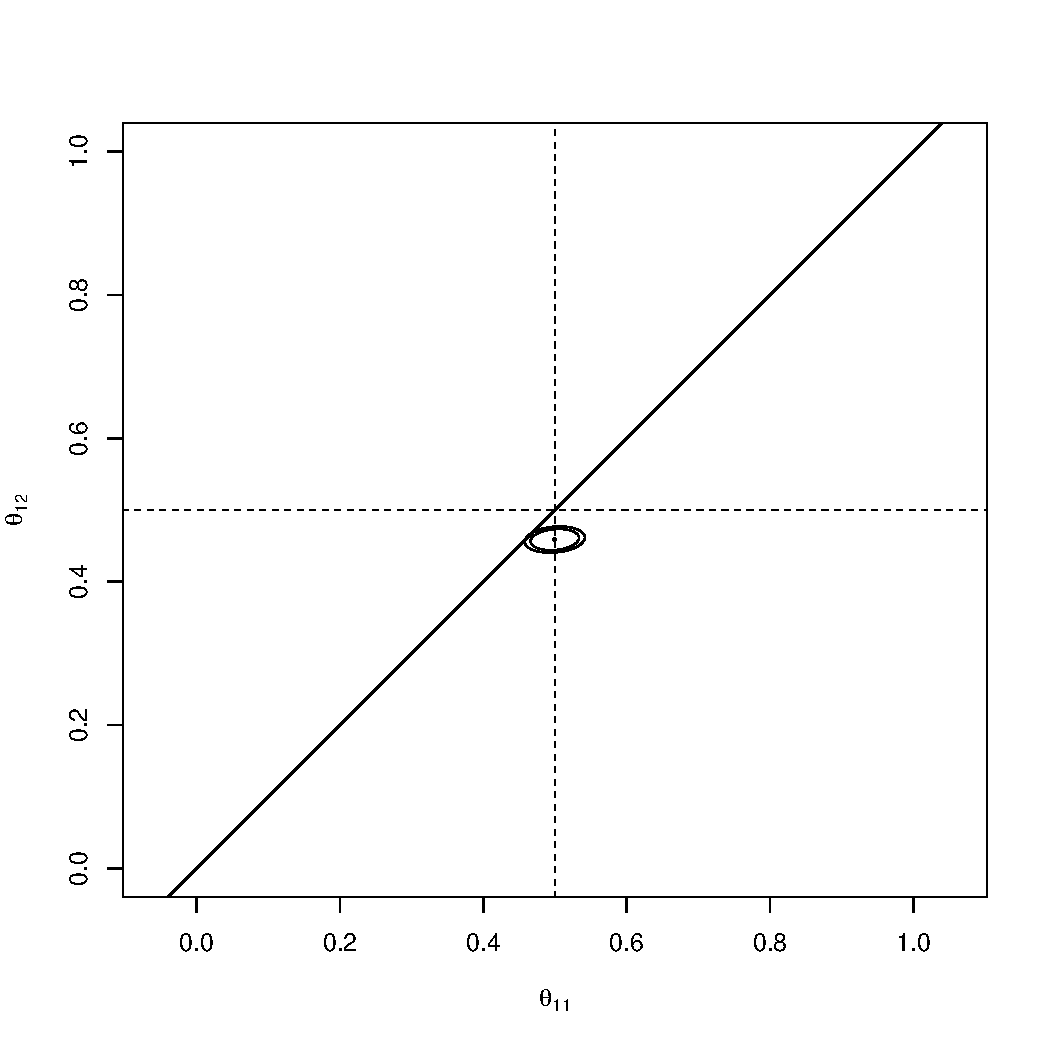
\includegraphics[width=0.5\textwidth]{220823_nyc.pdf}}
  \hfill
  \subfloat[Boston]{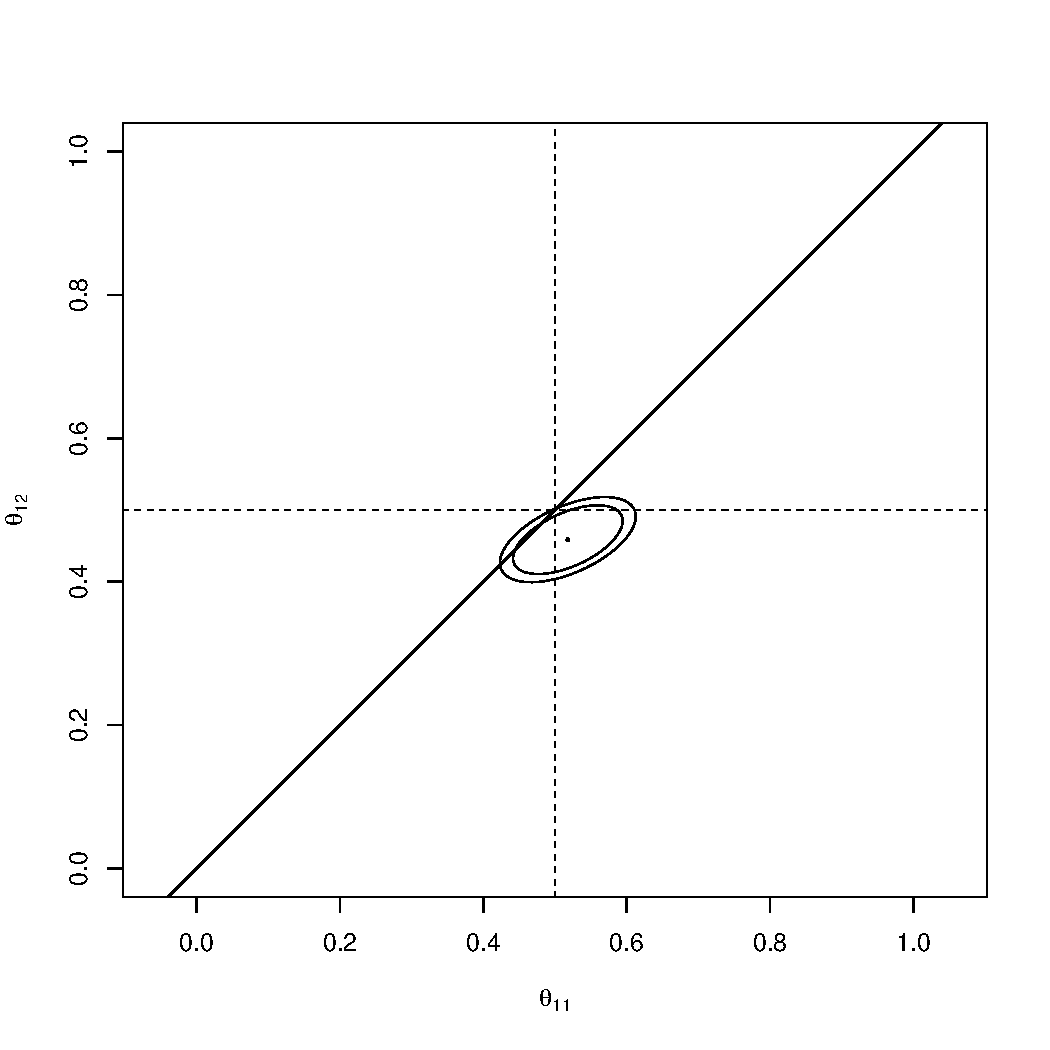
\includegraphics[width=0.5\textwidth]{220823_boston.pdf}}
  \caption{Level 95\% and 99\% Confidence ellipses for the estimates of $(\aucindiv,\aucpop)$ for duration of Terry stop by non-Black/Black status.}  \label{fig:data analysis:confidence ellipses}
\end{figure}



\bibliographystyle{apalike}
\bibliography{auc.bib}


\end{document}

possible additions:
1. conditions (eg location scale) that both theta12 and theta11 are $>1/2$ or $<1/2$ simultaneously. at least can't have delta depend on M,N.
2. maybe expand literature review
3. formulas for finite sample variance with gaussian data

questions about formatting:
1. proofs seem out of order because they numbering is by order of original proof statement.
2. spacing around large conditional bar

tell lu about obu simulation--doesnt have M,N/X,Y dependence



biometrics issues
parens
author postal address
25 p limit